% Options for packages loaded elsewhere
\PassOptionsToPackage{unicode}{hyperref}
\PassOptionsToPackage{hyphens}{url}
%
\documentclass[
]{article}
\usepackage{amsmath,amssymb}
\usepackage{iftex}
\ifPDFTeX
  \usepackage[T1]{fontenc}
  \usepackage[utf8]{inputenc}
  \usepackage{textcomp} % provide euro and other symbols
\else % if luatex or xetex
  \usepackage{unicode-math} % this also loads fontspec
  \defaultfontfeatures{Scale=MatchLowercase}
  \defaultfontfeatures[\rmfamily]{Ligatures=TeX,Scale=1}
\fi
\usepackage{lmodern}
\ifPDFTeX\else
  % xetex/luatex font selection
\fi
% Use upquote if available, for straight quotes in verbatim environments
\IfFileExists{upquote.sty}{\usepackage{upquote}}{}
\IfFileExists{microtype.sty}{% use microtype if available
  \usepackage[]{microtype}
  \UseMicrotypeSet[protrusion]{basicmath} % disable protrusion for tt fonts
}{}
\makeatletter
\@ifundefined{KOMAClassName}{% if non-KOMA class
  \IfFileExists{parskip.sty}{%
    \usepackage{parskip}
  }{% else
    \setlength{\parindent}{0pt}
    \setlength{\parskip}{6pt plus 2pt minus 1pt}}
}{% if KOMA class
  \KOMAoptions{parskip=half}}
\makeatother
\usepackage{xcolor}
\usepackage[margin=1in]{geometry}
\usepackage{color}
\usepackage{fancyvrb}
\newcommand{\VerbBar}{|}
\newcommand{\VERB}{\Verb[commandchars=\\\{\}]}
\DefineVerbatimEnvironment{Highlighting}{Verbatim}{commandchars=\\\{\}}
% Add ',fontsize=\small' for more characters per line
\usepackage{framed}
\definecolor{shadecolor}{RGB}{248,248,248}
\newenvironment{Shaded}{\begin{snugshade}}{\end{snugshade}}
\newcommand{\AlertTok}[1]{\textcolor[rgb]{0.94,0.16,0.16}{#1}}
\newcommand{\AnnotationTok}[1]{\textcolor[rgb]{0.56,0.35,0.01}{\textbf{\textit{#1}}}}
\newcommand{\AttributeTok}[1]{\textcolor[rgb]{0.13,0.29,0.53}{#1}}
\newcommand{\BaseNTok}[1]{\textcolor[rgb]{0.00,0.00,0.81}{#1}}
\newcommand{\BuiltInTok}[1]{#1}
\newcommand{\CharTok}[1]{\textcolor[rgb]{0.31,0.60,0.02}{#1}}
\newcommand{\CommentTok}[1]{\textcolor[rgb]{0.56,0.35,0.01}{\textit{#1}}}
\newcommand{\CommentVarTok}[1]{\textcolor[rgb]{0.56,0.35,0.01}{\textbf{\textit{#1}}}}
\newcommand{\ConstantTok}[1]{\textcolor[rgb]{0.56,0.35,0.01}{#1}}
\newcommand{\ControlFlowTok}[1]{\textcolor[rgb]{0.13,0.29,0.53}{\textbf{#1}}}
\newcommand{\DataTypeTok}[1]{\textcolor[rgb]{0.13,0.29,0.53}{#1}}
\newcommand{\DecValTok}[1]{\textcolor[rgb]{0.00,0.00,0.81}{#1}}
\newcommand{\DocumentationTok}[1]{\textcolor[rgb]{0.56,0.35,0.01}{\textbf{\textit{#1}}}}
\newcommand{\ErrorTok}[1]{\textcolor[rgb]{0.64,0.00,0.00}{\textbf{#1}}}
\newcommand{\ExtensionTok}[1]{#1}
\newcommand{\FloatTok}[1]{\textcolor[rgb]{0.00,0.00,0.81}{#1}}
\newcommand{\FunctionTok}[1]{\textcolor[rgb]{0.13,0.29,0.53}{\textbf{#1}}}
\newcommand{\ImportTok}[1]{#1}
\newcommand{\InformationTok}[1]{\textcolor[rgb]{0.56,0.35,0.01}{\textbf{\textit{#1}}}}
\newcommand{\KeywordTok}[1]{\textcolor[rgb]{0.13,0.29,0.53}{\textbf{#1}}}
\newcommand{\NormalTok}[1]{#1}
\newcommand{\OperatorTok}[1]{\textcolor[rgb]{0.81,0.36,0.00}{\textbf{#1}}}
\newcommand{\OtherTok}[1]{\textcolor[rgb]{0.56,0.35,0.01}{#1}}
\newcommand{\PreprocessorTok}[1]{\textcolor[rgb]{0.56,0.35,0.01}{\textit{#1}}}
\newcommand{\RegionMarkerTok}[1]{#1}
\newcommand{\SpecialCharTok}[1]{\textcolor[rgb]{0.81,0.36,0.00}{\textbf{#1}}}
\newcommand{\SpecialStringTok}[1]{\textcolor[rgb]{0.31,0.60,0.02}{#1}}
\newcommand{\StringTok}[1]{\textcolor[rgb]{0.31,0.60,0.02}{#1}}
\newcommand{\VariableTok}[1]{\textcolor[rgb]{0.00,0.00,0.00}{#1}}
\newcommand{\VerbatimStringTok}[1]{\textcolor[rgb]{0.31,0.60,0.02}{#1}}
\newcommand{\WarningTok}[1]{\textcolor[rgb]{0.56,0.35,0.01}{\textbf{\textit{#1}}}}
\usepackage{graphicx}
\makeatletter
\def\maxwidth{\ifdim\Gin@nat@width>\linewidth\linewidth\else\Gin@nat@width\fi}
\def\maxheight{\ifdim\Gin@nat@height>\textheight\textheight\else\Gin@nat@height\fi}
\makeatother
% Scale images if necessary, so that they will not overflow the page
% margins by default, and it is still possible to overwrite the defaults
% using explicit options in \includegraphics[width, height, ...]{}
\setkeys{Gin}{width=\maxwidth,height=\maxheight,keepaspectratio}
% Set default figure placement to htbp
\makeatletter
\def\fps@figure{htbp}
\makeatother
\setlength{\emergencystretch}{3em} % prevent overfull lines
\providecommand{\tightlist}{%
  \setlength{\itemsep}{0pt}\setlength{\parskip}{0pt}}
\setcounter{secnumdepth}{-\maxdimen} % remove section numbering
\ifLuaTeX
  \usepackage{selnolig}  % disable illegal ligatures
\fi
\IfFileExists{bookmark.sty}{\usepackage{bookmark}}{\usepackage{hyperref}}
\IfFileExists{xurl.sty}{\usepackage{xurl}}{} % add URL line breaks if available
\urlstyle{same}
\hypersetup{
  pdftitle={FE570 - Midterm Exam},
  pdfauthor={Sid Bhatia},
  hidelinks,
  pdfcreator={LaTeX via pandoc}}

\title{FE570 - Midterm Exam}
\usepackage{etoolbox}
\makeatletter
\providecommand{\subtitle}[1]{% add subtitle to \maketitle
  \apptocmd{\@title}{\par {\large #1 \par}}{}{}
}
\makeatother
\subtitle{I pledge my honor that I have abided by the Stevens Honor
System.}
\author{Sid Bhatia}
\date{2023-10-23}

\begin{document}
\maketitle

\subsection{Problem 11}\label{problem-11}

The data for this problem is contained in the file \emph{taqdata
BTCUSD.RData}. This is a trade-and-quote file giving the trade price,
size, and the quotes at the time of each trade for Bitcoin trades during
24 hours (19-Apr-2023).

\begin{Shaded}
\begin{Highlighting}[]
\CommentTok{\# Load necessary packages.}
\FunctionTok{library}\NormalTok{(xts)}
\end{Highlighting}
\end{Shaded}

\begin{verbatim}
## Loading required package: zoo
\end{verbatim}

\begin{verbatim}
## 
## Attaching package: 'zoo'
\end{verbatim}

\begin{verbatim}
## The following objects are masked from 'package:base':
## 
##     as.Date, as.Date.numeric
\end{verbatim}

\begin{verbatim}
## 
## ################################### WARNING ###################################
## # We noticed you have dplyr installed. The dplyr lag() function breaks how    #
## # base R's lag() function is supposed to work, which breaks lag(my_xts).      #
## #                                                                             #
## # If you call library(dplyr) later in this session, then calls to lag(my_xts) #
## # that you enter or source() into this session won't work correctly.          #
## #                                                                             #
## # All package code is unaffected because it is protected by the R namespace   #
## # mechanism.                                                                  #
## #                                                                             #
## # Set `options(xts.warn_dplyr_breaks_lag = FALSE)` to suppress this warning.  #
## #                                                                             #
## # You can use stats::lag() to make sure you're not using dplyr::lag(), or you #
## # can add conflictRules('dplyr', exclude = 'lag') to your .Rprofile to stop   #
## # dplyr from breaking base R's lag() function.                                #
## ################################### WARNING ###################################
\end{verbatim}

\begin{Shaded}
\begin{Highlighting}[]
\FunctionTok{library}\NormalTok{(highfrequency)}

\CommentTok{\# Load in data set.}
\FunctionTok{options}\NormalTok{(}\AttributeTok{digits.secs=}\DecValTok{3}\NormalTok{)}
\NormalTok{absolute\_path }\OtherTok{\textless{}{-}} \StringTok{\textquotesingle{}C:/Users/sbhatia2/My Drive/University/Academics/Semester V/FE570 {-} Market Microstructure and Trading Strategies/FE570 {-} Exams/FE570 {-} Midterm Exam/\textquotesingle{}}
\FunctionTok{load}\NormalTok{(}\FunctionTok{paste}\NormalTok{(absolute\_path, }\StringTok{"taqdata\_BTCUSD.RData"}\NormalTok{, }\AttributeTok{sep =} \StringTok{""}\NormalTok{))}

\CommentTok{\# Added to remove warnings about time zone mismatch.}
\FunctionTok{Sys.setenv}\NormalTok{(}\AttributeTok{TZ=}\StringTok{\textquotesingle{}GMT\textquotesingle{}}\NormalTok{)}

\FunctionTok{head}\NormalTok{(tqdata, }\DecValTok{10}\NormalTok{)}
\end{Highlighting}
\end{Shaded}

\begin{verbatim}
##                          DT SYMBOL   BID     OFR OFRSIZ BIDSIZ   PRICE
##  1: 2023-04-19 04:00:01.024 XBTUSD 30375 30375.5 189700  56200 30375.0
##  2: 2023-04-19 04:00:01.206 XBTUSD 30375 30375.5 189700  55600 30375.0
##  3: 2023-04-19 04:00:07.138 XBTUSD 30375 30375.5 224100  69300 30375.0
##  4: 2023-04-19 04:00:08.724 XBTUSD 30375 30375.5 227300  54800 30375.5
##  5: 2023-04-19 04:00:11.802 XBTUSD 30375 30375.5 226300  53100 30375.0
##  6: 2023-04-19 04:00:14.295 XBTUSD 30375 30375.5 227500  38600 30375.5
##  7: 2023-04-19 04:00:14.458 XBTUSD 30375 30375.5 227400  38600 30375.5
##  8: 2023-04-19 04:00:15.096 XBTUSD 30375 30375.5 222900  32700 30375.0
##  9: 2023-04-19 04:00:15.224 XBTUSD 30375 30375.5 222900  16200 30375.0
## 10: 2023-04-19 04:00:15.239 XBTUSD 30374 30375.0   7700   2500 30375.0
##     NUMTRADES  SIZE SIDE
##  1:         4 92900 Sell
##  2:         1   600 Sell
##  3:         1   900 Sell
##  4:         1   300  Buy
##  5:         1 16200 Sell
##  6:         1   100  Buy
##  7:         1   100  Buy
##  8:         1 20400 Sell
##  9:         3 21000 Sell
## 10:         2 17300 Sell
\end{verbatim}

\paragraph{i.}\label{i.}

Report the number of trades in the dataset, and the minimum and maximum
trade price during the time interval in the dataset.

\begin{Shaded}
\begin{Highlighting}[]
\CommentTok{\# Retrieve the number of trades in the dataset.}
\NormalTok{num\_of\_trades }\OtherTok{\textless{}{-}} \FunctionTok{nrow}\NormalTok{(tqdata)}
\NormalTok{num\_of\_trades}
\end{Highlighting}
\end{Shaded}

\begin{verbatim}
## [1] 58793
\end{verbatim}

\begin{Shaded}
\begin{Highlighting}[]
\NormalTok{price }\OtherTok{\textless{}{-}} \FunctionTok{as.numeric}\NormalTok{(tqdata}\SpecialCharTok{$}\NormalTok{PRICE)}

\CommentTok{\# Establish minimum and maximum prices quoted.}
\NormalTok{p\_min }\OtherTok{\textless{}{-}} \FunctionTok{min}\NormalTok{(price)}
\NormalTok{p\_max }\OtherTok{\textless{}{-}} \FunctionTok{max}\NormalTok{(price)}

\NormalTok{p\_min}
\end{Highlighting}
\end{Shaded}

\begin{verbatim}
## [1] 28534.75
\end{verbatim}

\begin{Shaded}
\begin{Highlighting}[]
\NormalTok{p\_max}
\end{Highlighting}
\end{Shaded}

\begin{verbatim}
## [1] 30407.5
\end{verbatim}

The number of trades is \(\mathbf{58793}\) with the minimum price at
\(\mathbf{28534.75}\) and maximum price at \(\mathbf{30407.50}\).

\paragraph{ii.}\label{ii.}

For each transaction, compute the spread measures:

\[\text{Quoted Spread}: qs_t = \text{Ask}_t - \text{Bid}_t\]

\[\text{Effective Spread}: es_t = 2d_t(p_t - \text{Mid}_t)\].

\begin{Shaded}
\begin{Highlighting}[]
\CommentTok{\# Compute the bids and asks for each transaction.}
\NormalTok{ask }\OtherTok{\textless{}{-}} \FunctionTok{as.numeric}\NormalTok{(tqdata}\SpecialCharTok{$}\NormalTok{OFR)}
\NormalTok{bid }\OtherTok{\textless{}{-}} \FunctionTok{as.numeric}\NormalTok{(tqdata}\SpecialCharTok{$}\NormalTok{BID)}

\CommentTok{\# Compute the quoted spread.}
\NormalTok{quoted\_spread }\OtherTok{\textless{}{-}}\NormalTok{ ask }\SpecialCharTok{{-}}\NormalTok{ bid}

\FunctionTok{head}\NormalTok{(quoted\_spread, }\DecValTok{50}\NormalTok{)}
\end{Highlighting}
\end{Shaded}

\begin{verbatim}
##  [1] 0.5 0.5 0.5 0.5 0.5 0.5 0.5 0.5 0.5 1.0 0.5 0.5 0.5 0.5 0.5 0.5 0.5 0.5 0.5
## [20] 1.5 1.5 5.0 0.5 0.5 0.5 1.0 1.5 0.5 0.5 1.0 1.5 3.5 3.5 0.5 0.5 0.5 0.5 3.0
## [39] 0.5 2.5 0.5 1.0 1.0 2.5 3.5 2.5 0.5 0.5 0.5 0.5
\end{verbatim}

\begin{Shaded}
\begin{Highlighting}[]
\FunctionTok{tail}\NormalTok{(quoted\_spread, }\DecValTok{50}\NormalTok{)}
\end{Highlighting}
\end{Shaded}

\begin{verbatim}
##  [1] 0.5 0.5 0.5 0.5 0.5 0.5 0.5 0.5 0.5 0.5 0.5 0.5 0.5 0.5 0.5 0.5 0.5 0.5 0.5
## [20] 0.5 0.5 0.5 0.5 0.5 0.5 4.5 8.5 0.5 0.5 0.5 8.0 5.0 1.0 0.5 0.5 0.5 7.0 0.5
## [39] 0.5 0.5 0.5 0.5 0.5 0.5 6.0 3.0 0.5 3.5 4.5 5.0
\end{verbatim}

\begin{Shaded}
\begin{Highlighting}[]
\CommentTok{\# Compute the mid prices (average of best bid and best ask prices).}
\NormalTok{mid }\OtherTok{\textless{}{-}}\NormalTok{ (ask }\SpecialCharTok{+}\NormalTok{ bid) }\SpecialCharTok{*} \FloatTok{0.5}

\CommentTok{\# Retrieve the trade sign for each transaction.}
\NormalTok{sign }\OtherTok{\textless{}{-}}\NormalTok{ tqdata}\SpecialCharTok{$}\NormalTok{SIDE}

\CommentTok{\# Convert the trade sign for a "Buy" and "Sell" to 1 and {-}1, respectively.}
\NormalTok{sign\_converted }\OtherTok{\textless{}{-}}\NormalTok{ sign}
\NormalTok{sign\_converted[sign\_converted }\SpecialCharTok{==} \StringTok{"Buy"}\NormalTok{] }\OtherTok{\textless{}{-}} \DecValTok{1}
\NormalTok{sign\_converted[sign\_converted }\SpecialCharTok{==} \StringTok{"Sell"}\NormalTok{] }\OtherTok{\textless{}{-}} \SpecialCharTok{{-}}\DecValTok{1}

\NormalTok{sign\_converted }\OtherTok{\textless{}{-}} \FunctionTok{as.numeric}\NormalTok{(sign\_converted)}

\FunctionTok{head}\NormalTok{(sign, }\DecValTok{10}\NormalTok{)}
\end{Highlighting}
\end{Shaded}

\begin{verbatim}
##  [1] "Sell" "Sell" "Sell" "Buy"  "Sell" "Buy"  "Buy"  "Sell" "Sell" "Sell"
\end{verbatim}

\begin{Shaded}
\begin{Highlighting}[]
\FunctionTok{head}\NormalTok{(sign\_converted, }\DecValTok{10}\NormalTok{)}
\end{Highlighting}
\end{Shaded}

\begin{verbatim}
##  [1] -1 -1 -1  1 -1  1  1 -1 -1 -1
\end{verbatim}

\begin{Shaded}
\begin{Highlighting}[]
\CommentTok{\# Calculate the effective spread.}
\NormalTok{effective\_spread }\OtherTok{\textless{}{-}} \DecValTok{2} \SpecialCharTok{*}\NormalTok{ sign\_converted }\SpecialCharTok{*}\NormalTok{ (price }\SpecialCharTok{{-}}\NormalTok{ mid)}

\FunctionTok{head}\NormalTok{(effective\_spread, }\DecValTok{50}\NormalTok{)}
\end{Highlighting}
\end{Shaded}

\begin{verbatim}
##  [1]  0.5  0.5  0.5  0.5  0.5  0.5  0.5  0.5  0.5 -1.0  0.5  0.5  0.5  0.5 -0.5
## [16] -0.5  0.5  0.5  0.5 -0.5 -0.5 -4.0  0.5  0.5  0.5  0.0 -0.5  0.5  0.5  0.0
## [31]  0.5  3.5  3.5  0.5  0.5  0.5  0.5 -2.0  0.5 -1.5  0.5  0.0  0.0 -1.5  1.5
## [46] -1.5  0.5  0.5  0.5  0.5
\end{verbatim}

\begin{Shaded}
\begin{Highlighting}[]
\FunctionTok{tail}\NormalTok{(effective\_spread, }\DecValTok{50}\NormalTok{)}
\end{Highlighting}
\end{Shaded}

\begin{verbatim}
##  [1]  0.5  0.5  0.5  0.5  0.5  0.5  0.5  0.5  0.5  0.5  0.5  0.5  0.5  0.5 -0.5
## [16]  0.5  0.5  0.5  0.5  0.5  0.5  0.5  0.5  0.5  0.5  0.0  6.0  0.5  0.5  0.5
## [31]  0.0  0.0  1.0  0.5  0.5  0.5  3.5  0.5  0.5  0.5  0.5  0.5  0.5  0.5  1.0
## [46]  3.0  0.5 -2.5 -3.5 -3.0
\end{verbatim}

\begin{Shaded}
\begin{Highlighting}[]
\FunctionTok{mean}\NormalTok{(quoted\_spread)}
\end{Highlighting}
\end{Shaded}

\begin{verbatim}
## [1] 4.816764
\end{verbatim}

\begin{Shaded}
\begin{Highlighting}[]
\FunctionTok{mean}\NormalTok{(effective\_spread)}
\end{Highlighting}
\end{Shaded}

\begin{verbatim}
## [1] 1.956644
\end{verbatim}

The average quoted spread is \(\mathbf{4.817}\) and the average
effective spread is \(\mathbf{1.957}\).

\paragraph{iii.}\label{iii.}

Compute the Roll's estimate of the bid-ask spread.

\begin{Shaded}
\begin{Highlighting}[]
\CommentTok{\# Calculate the difference in price changes.}
\NormalTok{dprice }\OtherTok{\textless{}{-}} \FunctionTok{diff}\NormalTok{(price)}

\CommentTok{\# Compute and plot the autocorrelation of price changes.}
\NormalTok{ac\_pr }\OtherTok{\textless{}{-}} \FunctionTok{acf}\NormalTok{(dprice, }\AttributeTok{lag.max=}\DecValTok{20}\NormalTok{, }\AttributeTok{type=}\StringTok{"correlation"}\NormalTok{, }\AttributeTok{plot=}\ConstantTok{FALSE}\NormalTok{)}
\FunctionTok{plot}\NormalTok{(ac\_pr, }\AttributeTok{col=}\StringTok{"red"}\NormalTok{, }\AttributeTok{main=}\StringTok{"Autocorrelation of Price Changes"}\NormalTok{)}
\end{Highlighting}
\end{Shaded}

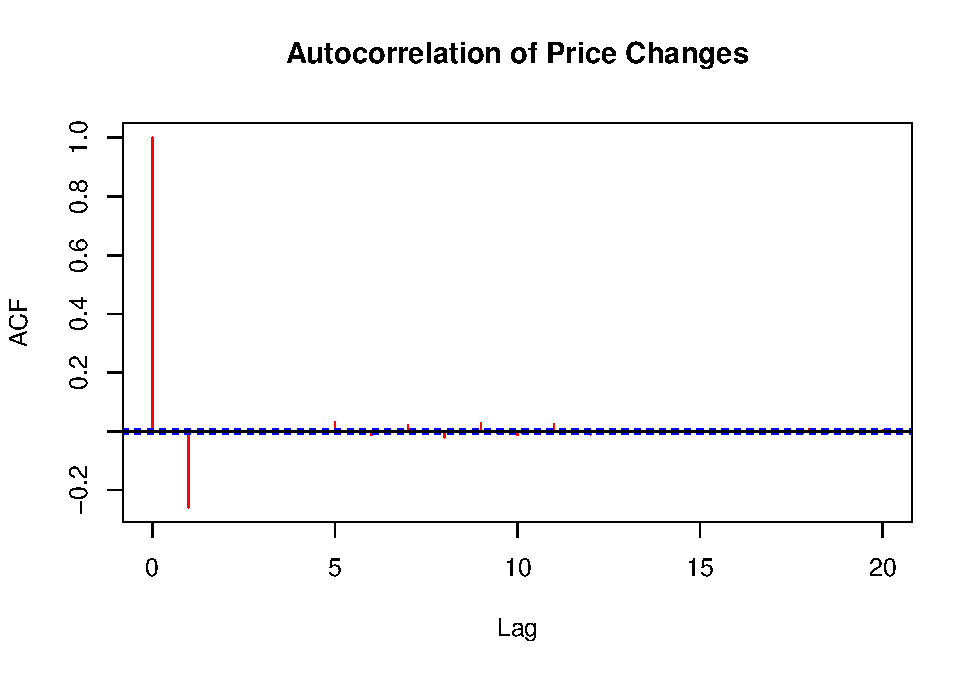
\includegraphics{FE570---MIdterm-Exam_files/figure-latex/unnamed-chunk-4-1.pdf}

\begin{Shaded}
\begin{Highlighting}[]
\CommentTok{\# Compute the covariances of the price changes.}
\NormalTok{covpr }\OtherTok{\textless{}{-}} \FunctionTok{acf}\NormalTok{(dprice, }\AttributeTok{lag.max=}\DecValTok{20}\NormalTok{, }\AttributeTok{type=}\StringTok{"covariance"}\NormalTok{, }\AttributeTok{plot=}\ConstantTok{FALSE}\NormalTok{)}

\CommentTok{\# Retrieve gamma1 as the covariance at lag 0.}
\NormalTok{gamma0 }\OtherTok{\textless{}{-}}\NormalTok{ covpr}\SpecialCharTok{$}\NormalTok{acf[}\DecValTok{1}\NormalTok{]}
\NormalTok{gamma0}
\end{Highlighting}
\end{Shaded}

\begin{verbatim}
## [1] 21.90887
\end{verbatim}

\begin{Shaded}
\begin{Highlighting}[]
\CommentTok{\# Retrieve gamma1 as the covariance at lag 1.}
\NormalTok{gamma1 }\OtherTok{\textless{}{-}}\NormalTok{ covpr}\SpecialCharTok{$}\NormalTok{acf[}\DecValTok{2}\NormalTok{]}
\NormalTok{gamma1}
\end{Highlighting}
\end{Shaded}

\begin{verbatim}
## [1] -5.655469
\end{verbatim}

\begin{Shaded}
\begin{Highlighting}[]
\CommentTok{\# Compute the volatility of the efficient price.}
\NormalTok{sig2u }\OtherTok{\textless{}{-}}\NormalTok{ gamma0 }\SpecialCharTok{+} \DecValTok{2} \SpecialCharTok{*}\NormalTok{ gamma1}
\NormalTok{sigu }\OtherTok{\textless{}{-}} \FunctionTok{sqrt}\NormalTok{(sig2u)}
\NormalTok{sigu}
\end{Highlighting}
\end{Shaded}

\begin{verbatim}
## [1] 3.255447
\end{verbatim}

\begin{Shaded}
\begin{Highlighting}[]
\CommentTok{\# Compute the c paramater as the sqrt({-}gamma1)}
\NormalTok{cparam }\OtherTok{\textless{}{-}} \FunctionTok{sqrt}\NormalTok{(}\SpecialCharTok{{-}}\NormalTok{gamma1)}
\NormalTok{cparam}
\end{Highlighting}
\end{Shaded}

\begin{verbatim}
## [1] 2.378123
\end{verbatim}

\begin{Shaded}
\begin{Highlighting}[]
\CommentTok{\# Compute the spread as 2 * the c parameter.}
\NormalTok{roll\_spread }\OtherTok{\textless{}{-}}\NormalTok{ cparam }\SpecialCharTok{*} \DecValTok{2}

\NormalTok{roll\_spread}
\end{Highlighting}
\end{Shaded}

\begin{verbatim}
## [1] 4.756246
\end{verbatim}

As such, the Roll's model estimate of the bid-ask spread is
\(\mathbf{4.756}\) with \(c = 2.378\) and \(\sigma_u = 3.255\).

\paragraph{iv.}\label{iv.}

Compare the trade sign in SIDE with the prediction of the Lee-Ready
empirical rule.

What is the accuracy of the Lee-Ready rule?

This can be measured as the percentage of trade signs which are
predicted correctly by the Lee-Ready rule.

\textbf{Tick Test}: Use only the trade prices \(p_t\), but not the
quotes \(a_t\) and \(b_t\). Under the test, the trade is classified as a
buy/sell according to: - \(d_t = +1\) (buy) if \(p_t > p_{t-1}\)
(uptick) or if \(p_t = p_{t-1} > p_{t-2}\) (zero-uptick) - \(d_t = -1\)
(sell) if \(p_t < p_{t-1}\) (downtick) or if \(p_t = p_{t-1} < p_{t-2}\)
(zero-downtick)

Note that zero-uptick/downtick results apply also if there are multiple
(more than 2) trades with the same price.

For example if the trade prices are \(p_t = (19.9, 20.0, 20.0, 20.0)\)
(increasing \(t\) order), then the trade signs are (?, +, + , +).

\textbf{Lee-Ready Rule}: Use both \(p_t\) and quotes \(a_t\) and
\(b_t\). The Lee-Ready Rule decides if a trade is a buy or sell by
comparing the trade price \(p_t\) with the mid-price
\(m_t = \frac{1}{2} (a_t + b_t)\) (the half-point between best-bid
\(b_t\) and best-ask \(a_t\)).

If the trade price is exactly equal to the mid-price, \(p_t = m_t\),
then use the tick rule in point (i) above.

\begin{Shaded}
\begin{Highlighting}[]
\CommentTok{\# Create a function that implements the Tick Test.}
\NormalTok{tick\_test }\OtherTok{\textless{}{-}} \ControlFlowTok{function}\NormalTok{(price)}
\NormalTok{\{}
\NormalTok{    sign }\OtherTok{\textless{}{-}} \FunctionTok{c}\NormalTok{(}\DecValTok{1}\NormalTok{)}
    \ControlFlowTok{for}\NormalTok{(i }\ControlFlowTok{in} \DecValTok{2}\SpecialCharTok{:}\NormalTok{(}\FunctionTok{length}\NormalTok{(price))) }
\NormalTok{    \{}
        \ControlFlowTok{if}\NormalTok{(price[i] }\SpecialCharTok{\textless{}}\NormalTok{ price[i }\SpecialCharTok{{-}} \DecValTok{1}\NormalTok{])}
\NormalTok{        \{}
\NormalTok{            sign }\OtherTok{\textless{}{-}} \FunctionTok{c}\NormalTok{(sign, }\SpecialCharTok{{-}}\DecValTok{1}\NormalTok{)}
\NormalTok{        \}}
        \ControlFlowTok{else} \ControlFlowTok{if}\NormalTok{(price[i] }\SpecialCharTok{\textgreater{}}\NormalTok{ price[i }\SpecialCharTok{{-}} \DecValTok{1}\NormalTok{])}
\NormalTok{        \{}
\NormalTok{            sign }\OtherTok{\textless{}{-}} \FunctionTok{c}\NormalTok{(sign, }\DecValTok{1}\NormalTok{)}
\NormalTok{        \}}
        \ControlFlowTok{else}
\NormalTok{        \{}
\NormalTok{            sign }\OtherTok{\textless{}{-}} \FunctionTok{c}\NormalTok{(sign, sign[i }\SpecialCharTok{{-}} \DecValTok{1}\NormalTok{])}
\NormalTok{        \}}
\NormalTok{    \}}
    \FunctionTok{return}\NormalTok{(sign)}
\NormalTok{\}}

\CommentTok{\# Create a function that implements the Lee{-}Ready Rule.}
\NormalTok{lee\_ready\_rule }\OtherTok{\textless{}{-}} \ControlFlowTok{function}\NormalTok{(price)}
\NormalTok{\{}
\NormalTok{    tick }\OtherTok{\textless{}{-}} \FunctionTok{tick\_test}\NormalTok{(price)}
\NormalTok{    sign }\OtherTok{\textless{}{-}} \FunctionTok{c}\NormalTok{(}\DecValTok{1}\NormalTok{)}
\NormalTok{    bid }\OtherTok{\textless{}{-}} \FunctionTok{sapply}\NormalTok{(tqdata}\SpecialCharTok{$}\NormalTok{BID, }\AttributeTok{FUN =}\NormalTok{ as.numeric)}
\NormalTok{    ask }\OtherTok{\textless{}{-}} \FunctionTok{sapply}\NormalTok{(tqdata}\SpecialCharTok{$}\NormalTok{OFR, }\AttributeTok{FUN =}\NormalTok{ as.numeric)}

    \ControlFlowTok{for}\NormalTok{(i }\ControlFlowTok{in} \DecValTok{2}\SpecialCharTok{:}\NormalTok{(}\FunctionTok{length}\NormalTok{(price)))}
\NormalTok{    \{}
\NormalTok{        mid }\OtherTok{\textless{}{-}}\NormalTok{ (bid[i] }\SpecialCharTok{+}\NormalTok{ ask[i]) }\SpecialCharTok{*} \FloatTok{0.5}

        \ControlFlowTok{if}\NormalTok{(price[i] }\SpecialCharTok{\textgreater{}}\NormalTok{ mid)}
\NormalTok{        \{}
\NormalTok{            sign }\OtherTok{\textless{}{-}} \FunctionTok{c}\NormalTok{(sign, }\DecValTok{1}\NormalTok{)}
\NormalTok{        \}}
        \ControlFlowTok{else} \ControlFlowTok{if}\NormalTok{(price[i] }\SpecialCharTok{\textless{}}\NormalTok{ mid)}
\NormalTok{        \{}
\NormalTok{            sign }\OtherTok{\textless{}{-}} \FunctionTok{c}\NormalTok{(sign, }\SpecialCharTok{{-}}\DecValTok{1}\NormalTok{)}
\NormalTok{        \}}
        \ControlFlowTok{else} 
\NormalTok{        \{}
\NormalTok{            sign }\OtherTok{\textless{}{-}} \FunctionTok{c}\NormalTok{(sign, tick[i])}
\NormalTok{        \}}
\NormalTok{    \}}
    \FunctionTok{return}\NormalTok{(sign)}
\NormalTok{\}}

\NormalTok{Lee\_Ready\_Rule\_TQ }\OtherTok{\textless{}{-}} \FunctionTok{lee\_ready\_rule}\NormalTok{(price)}

\NormalTok{Lee\_Ready\_Rule\_Actual }\OtherTok{\textless{}{-}} \FunctionTok{getTradeDirection}\NormalTok{(tqdata)}

\CommentTok{\# Check to see if Lee{-}Ready implementation is the same.}
\FunctionTok{length}\NormalTok{( }\FunctionTok{which}\NormalTok{(Lee\_Ready\_Rule\_Actual }\SpecialCharTok{==}\NormalTok{ Lee\_Ready\_Rule\_TQ ) ) }\SpecialCharTok{/} \FunctionTok{length}\NormalTok{(Lee\_Ready\_Rule\_TQ)}
\end{Highlighting}
\end{Shaded}

\begin{verbatim}
## [1] 0.999983
\end{verbatim}

\begin{Shaded}
\begin{Highlighting}[]
\CommentTok{\# Check to see accuracy of Lee{-}Ready Rule.}
\FunctionTok{length}\NormalTok{( }\FunctionTok{which}\NormalTok{(sign\_converted }\SpecialCharTok{==}\NormalTok{  Lee\_Ready\_Rule\_Actual) ) }\SpecialCharTok{/} \FunctionTok{length}\NormalTok{(sign\_converted)}
\end{Highlighting}
\end{Shaded}

\begin{verbatim}
## [1] 0.7426564
\end{verbatim}

\begin{Shaded}
\begin{Highlighting}[]
\FunctionTok{length}\NormalTok{( }\FunctionTok{which}\NormalTok{(sign\_converted }\SpecialCharTok{==}\NormalTok{  Lee\_Ready\_Rule\_TQ) ) }\SpecialCharTok{/} \FunctionTok{length}\NormalTok{(sign\_converted)}
\end{Highlighting}
\end{Shaded}

\begin{verbatim}
## [1] 0.7426394
\end{verbatim}

As such, the Lee-Ready rule is \(74.3\%\) accurate in terms of the trade
signs it correctly predicted.

\end{document}
